\begin{quote}
	计算机系统中没有魔法. \hfill -- 蒋炎岩
\end{quote}



\section{数据与数据结构}

\ti{中学的练习题与计算机中的算法}

计算机的一个重要的功能是存储和操作数据. 那么从“数据”的角度看,通过算法希望计算机帮我们解的“题”与你们中学数学课上解的题有什么不同?

事实上, 算法的输入是满足特定条件的对象的集合(“问题空间”),算法必须能保证对该集合中“任一对象”均能计算出正确的结果。程序是算法的“实现”,其“每一次”执行处理的是某个特定数据对象(问题实例)。

因此,中学数学课中的那些“题目”是我们这里讨论的算法问题的“实例”。因为我们只需要对于单一的个体进行回答. 

对于算法而言, 为什么讨论计算机问题求解必须讨论“数据”?首先, 输入数据必须以某种形式“放入”计算机;输出结果必须以某种形式的数据呈现给用户;问题求解过程可以看作“数据转换”过程,这个过程如果有多个步骤组成,则每个步骤可能需要以中间形式暂时存放,供后面的步骤使用。

最基本的数据可以说为变量了. 在第一章中, 我们说明了我们认为变量是存储一个``东西''的盒子. 我们说这个``盒子''其实有两种形式. 按值(by value)或者按引用(by reference). 见图. 

% TODO. 补充by value和by reference的图

比如, 在“冒泡”排序算法中,核心操作是“交换序列中两个元素(不妨说是$x$,$y$),其实现过程可以表示如下(注意:需要使用一个临时辅助变量$z$):
$$
\begin{aligned}
z&\leftarrow x\\
x&\leftarrow y\\
y&\leftarrow z	
\end{aligned}
$$

在C语言中, 为什么对变量要指定“类型”?首先, 变量的类型表示了这些变量够执行什么样的“操作”(运算). 我们为什么要给变量起名字? 其实变量名的本质在于. 变(常)量名是计算机存储区地址的“抽象”. 编程时关注的“位置”与计算机内的物理地址无关.

在数据结构中, “结构”究竟是什么?实际上, 控制结构与数据结构是计算机算法的两个侧面,数据结构不仅仅是关乎数据“如何放”。

\begin{quote}
	While \blue{control structures} serve to tell the processor \blue{where it should be going}, \red{data structures}, and the operations upon them, organize the data items in ways that enable it to \red{do whatever it should do} when it gets there.
\end{quote}

比如, “全班同学排好队!”是什么意思?首先, 每人有了一个“位置”。然后, 其实这个“位置”是相对的。其实, 如果安排一种按照位置进行的“游戏”,“到了什么位置就知道该做什么”。

这样我们就知道了程序设计语言中的数组到底是什么. 数组就相当于抽象的逻辑结构是“顺序”结构. 在计算机中的“实现”就是同类型数据的“序列”。程序设计语言为你提供了定义特定数组的“设施”. 物理位置就可以不用管了. 

我们选取的数据结构与控制结构的对应(图\ref{figs:cflow}). 来看几个例子. 

\begin{figure}
	\centering
	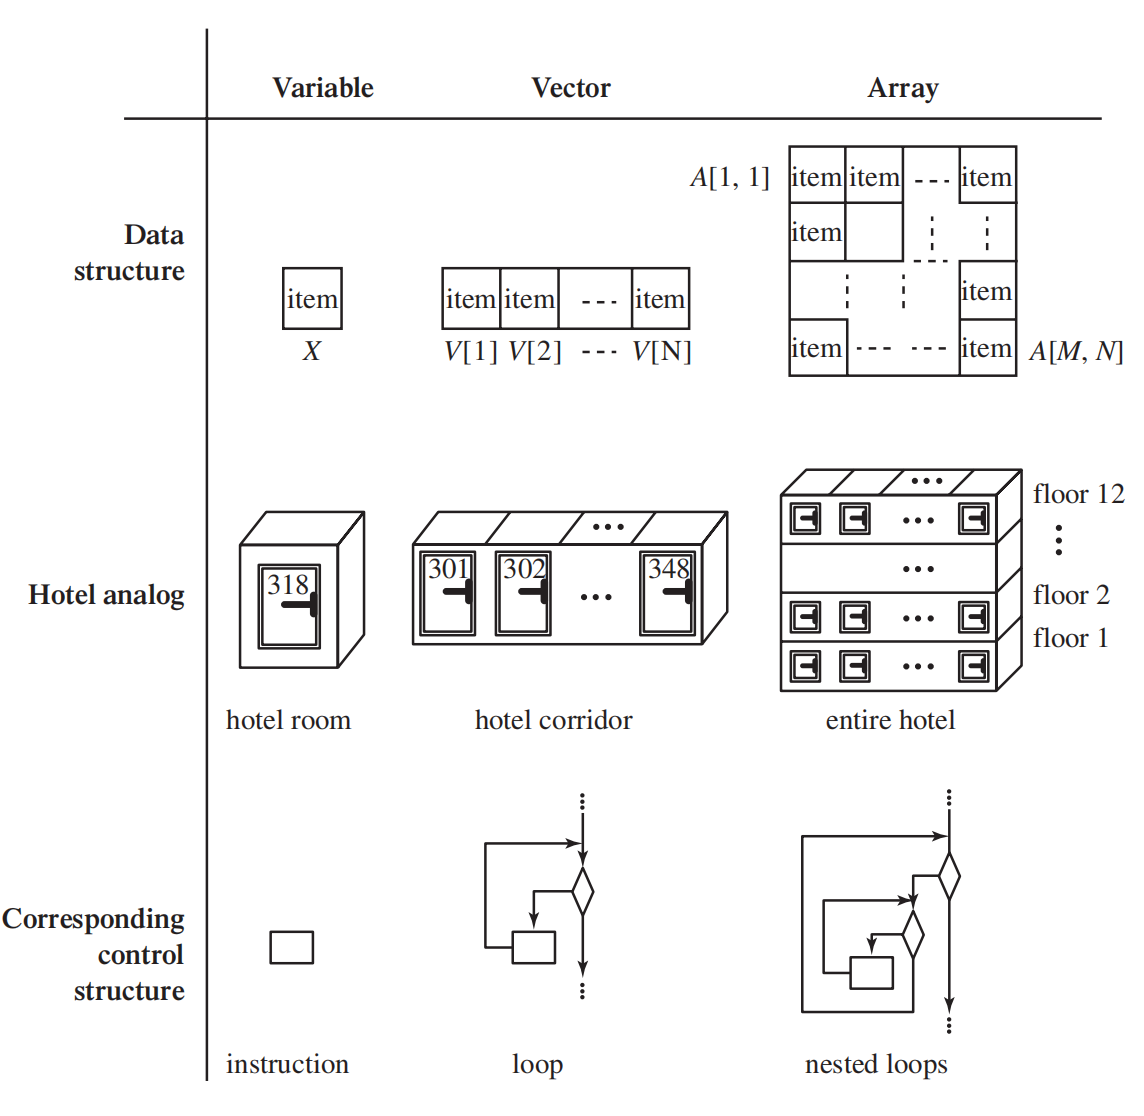
\includegraphics[scale=0.5]{4-programs/figs/structures}
	\caption{数据结构与控制结构的对应的例子}
	\label{figs:cflow}
	
\end{figure}

比如, 我们写了一个$n$维的数组, 但是可能想过, 数组维数的相对性. 比如一个二维数组可以写称为vector套vector. 

这就是数组的一些有趣的事情. 下面来总结一下. 数组结构的访问方式特点是什么,对于解题有什么好处?又带来什么不便?

数组元素使用“下标”确定其位置,而下标是顺序编排的,这对访问数组元素带来什么便利?正因为顺序编排,对于在应用中如果需要增删元素则必须“维护”相应的特性?

你若需要对数组元素进行如下操作,可能必须移动“整块”的其它元素:(1)在指定位置插入一个新元素;(2)删除某个位置上的元素但不留下“空挡”, 那么代价可能很大. 

数组实际上是通过连续编排下标将元素顺序连接成一个“结构”. 如果我们将“顺序连接”抽象为对用户“透明”的实现方式,那么数组就可以认为是“抽象数据类型”list的一种实现。list中“顺序”的概念是抽象的,可以用不同方式实现. 常用的linked-list可以认为是一种使用“指针”的实现。显然linked-list(链表)可以解决数组的不便。而且更适用于执行前无法确定序列长度的情况。

我们发现我们不关心这里面的数据到底是什么. 所谓“抽象数据类型”不涉及数据对象的性质以及其“存放”方式,仅通过操作定义体现在“解题”时的应用意义。比如, 简化的list由4个操作定义:(1)一个创建(插入)操作,两个“查询”操作,一个常量.

\begin{lstlisting}
list cons(obj newElement, oldList)
Precondition: none
Postcondition: if x=con(newElement, oldList)  then:
    (1) x refer to a newly created list
    (2) x!=nil
    (3) first(x)=newElement
    (4) rest(x)=oldList
obj first(list aList)
Precondition: aList!=nil

list rest(list aList)
Precondition: sList!=nil

list nil
\end{lstlisting}


\ti{抽象数据类型与问题求解}

我们来考察如下的两个情形: (1)在图书馆的书架某一层取一本书; (2) 在机场的饮水机旁取一个纸杯. 这两者有何不同?其实, 如果仅仅从“放置”的角度看,两者涉及的物体放置方式是一样的:“一个挨着一个的顺序结构”,不同的是对元素的操作方式。我们的操作方式是被受到限制的. 即使一样的“受限”操作方式,也可以有不同的“限”法:比如栈(stack)和队列(queue)在不同的问题的求解有不同的明显的意义。


比如判定输入字符串是否“回文(palindrome)”也就是从头读到尾与从尾读到头完全一样. 一个最朴素的想法就是通过数组的方式存储每一个字符, 然后正着倒着循环并且判断即可. 另一个例子是模拟一个排队的场景: 设想一个单服务柜台的运行状态,设定模拟总时间长度,随机生成“新顾客到达时间及其需要的服务处理时长”模拟可能的排队等待队列人数变化情况。假设服务能力与预期顾客需求量总量平衡。既然是``队列'', 我们就不允许新元素``插队''了. 

想一想大学里面选修课程的依赖, 以及家谱(family tree), 它们一般构成一个树的关系--这样非线性的内容是如何存在计算机中的呢? 事实上, 我们并不是真正的在内存里按照图形的样子进行存储的. 我们是使用引用的方式来把这个关系搞清楚的. 树的一个比较明显的特征是可分“层”. 

我们在内存里面是如何存储树的呢? 事实上, 我们只要在每个节点上打上它儿子节点的编号就行了. 这样我们在找子树的时候就可以按照编号去对应的位置去寻找了. 当然这只是一种方法, 其他的方法大同小异, 不过这样一个对应关系还是绕不过去的. 

\begin{figure}[h!]
	\centering
	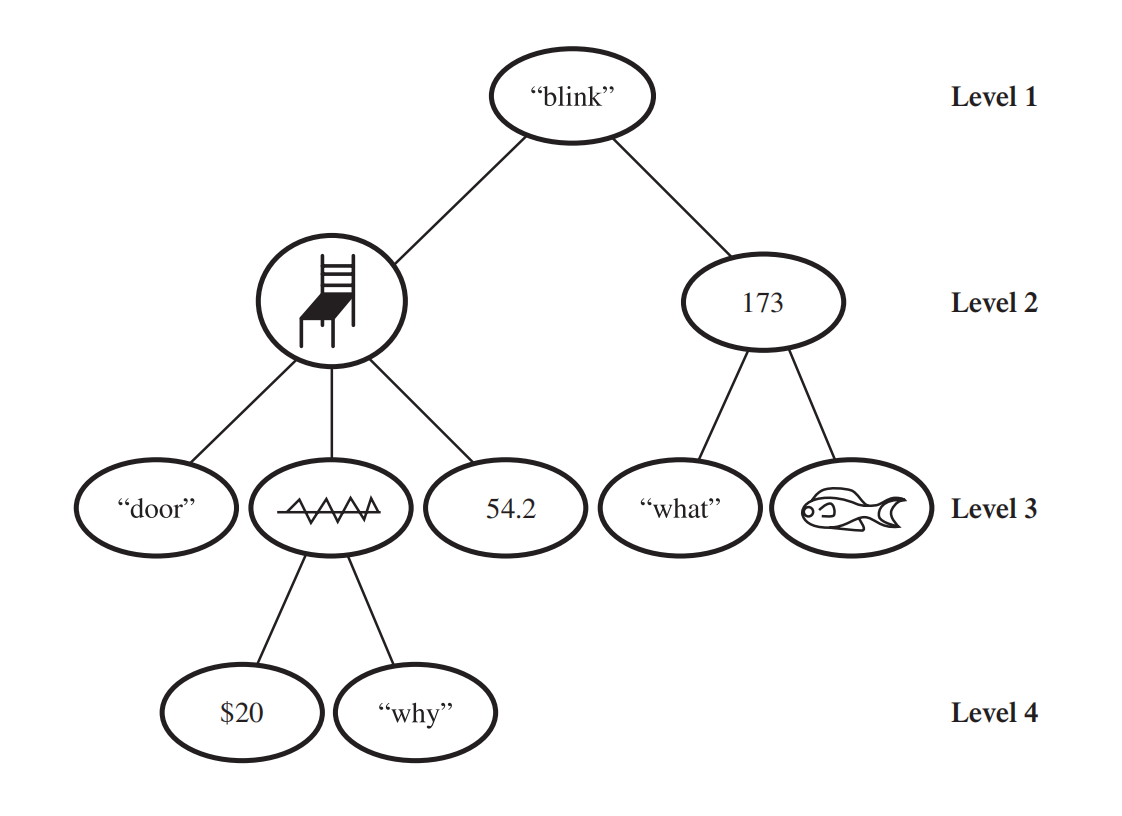
\includegraphics[scale=0.5]{4-programs/figs/tree}
	\caption{一棵``树''}
	\label{figs:tree-fig}
	
\end{figure}

如果这里是一个数组或者嵌套的数组, 我们可以很容易的看到它里面的所有的元素是什么. 那么如果是树我们应该如何看到它的内容呢? 

这就要回到我们如何看树了. 从非递归的视角来看, 我们有一个“结点”的集合$\set{A,B,\cdots,K}$, 以及一个“独特”的结点 – “根”:$A$. 根只有“出边”,没有“入边”. 其它任何结点有恰好一个“入边”, 这也就保证了每一个节点具有唯一的通路.  从递归视角来看, 会发现它有一个唯一的“根”结点. 假设根结点有$k$条出边,其另一端点为 $v_1,v_2,\cdots,v_k$,它们分别是$k$个无结点相交的树的根,这些树称为“子树”. 

从递归的视角来看树可以由很多的好处. 比如, 这就可以让我们发现如果要遍历一棵树, 那么先遍历左边子树, 在遍历右边的子树就行了. 这看上去比较抽象, 我们下面说几个比较有趣的例子. 

\textbf{例子1. 利用树排序. }(见图\ref{figs:tree-sort}) 首先, 将数组表示为“二分搜索树”. ``二分搜索树''的生成方式是这样的: 每个节点的左边节点的数值一定比它的值小, 右边的一定比它的值大. 以“深度优先”方式遍历树, 那么输出方式一定是从小到大的. 


\begin{figure}[h!]
	\centering
	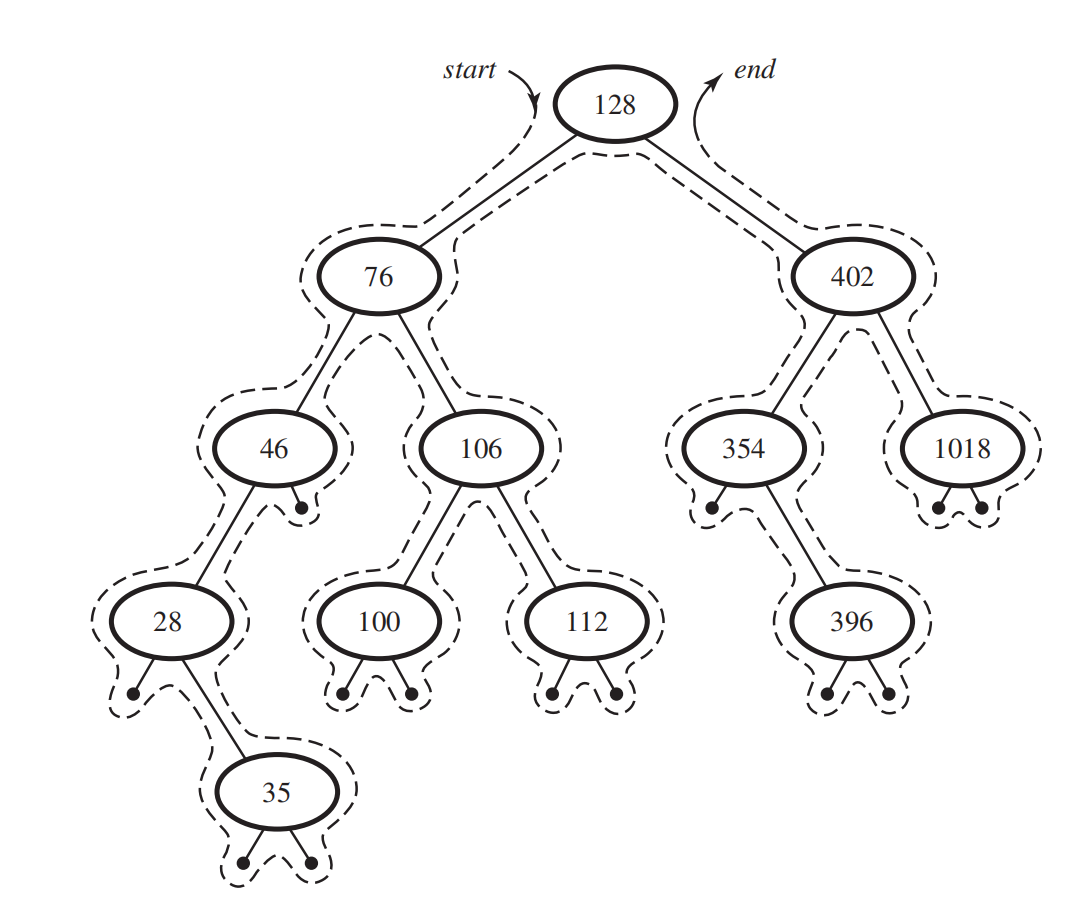
\includegraphics[scale=0.8]{4-programs/figs/tree-sort.png}
	\caption{用于排序的树}
	\label{figs:tree-sort}
	
\end{figure}

\textbf{例子2. 树结构和算数表达求值. }(见图\ref{figs:tree-eval}) 如算术表达式:$(10 + (( 22 – 3 \times 4) / 2 – 2 \times 2 ) \times (( 14 – 2) / (1 + 3 ) )$. 对应的表达式树就是这样的: 

\begin{figure}[h!]
	\centering
	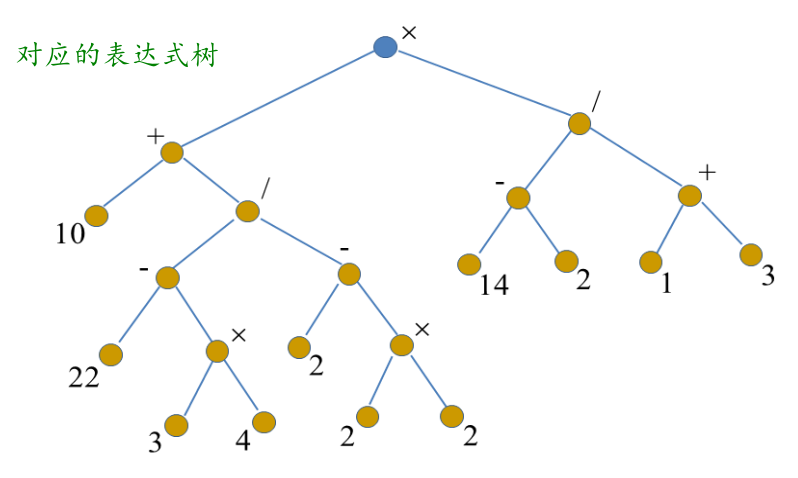
\includegraphics[scale=0.8]{4-programs/figs/exptree}
	\caption{由于表达式求值的树}
	\label{figs:tree-eval}
	
\end{figure}


我们使用Left-first traversal(Third-visit output, 称为“后序”). 

其实还有一个新的方法: 假如数字输出到一个堆栈中,每当遇到运算符则处理前面两个数,结果仍然是对的. 


\section{把算法告诉计算机}
\ti{从算法到程序}

我们可能会说, 把算法告诉计算机有什么难的? 写点代码就行了啊! 但计算机的最底层是01的组合, 我们今天并没有用0,1表述我们的算法. 

事实上, “早期”的程序员真的用0, 1编程序. 他们使用的是打孔纸带和操作系统进行. 其一般有三个部分组成. 如图\ref{figs:prog-early}. 就是一条条这样的“指令”用来告诉物理的电路要做什么: 哪个开关打开, 哪个应该关闭. 计算机虽然能接受这样的语言表述,但并不知道你究竟“想干什么”--因为“编程自动化”远比“算法设计自动化”要容易! 

\begin{figure}[h!]
	\centering
	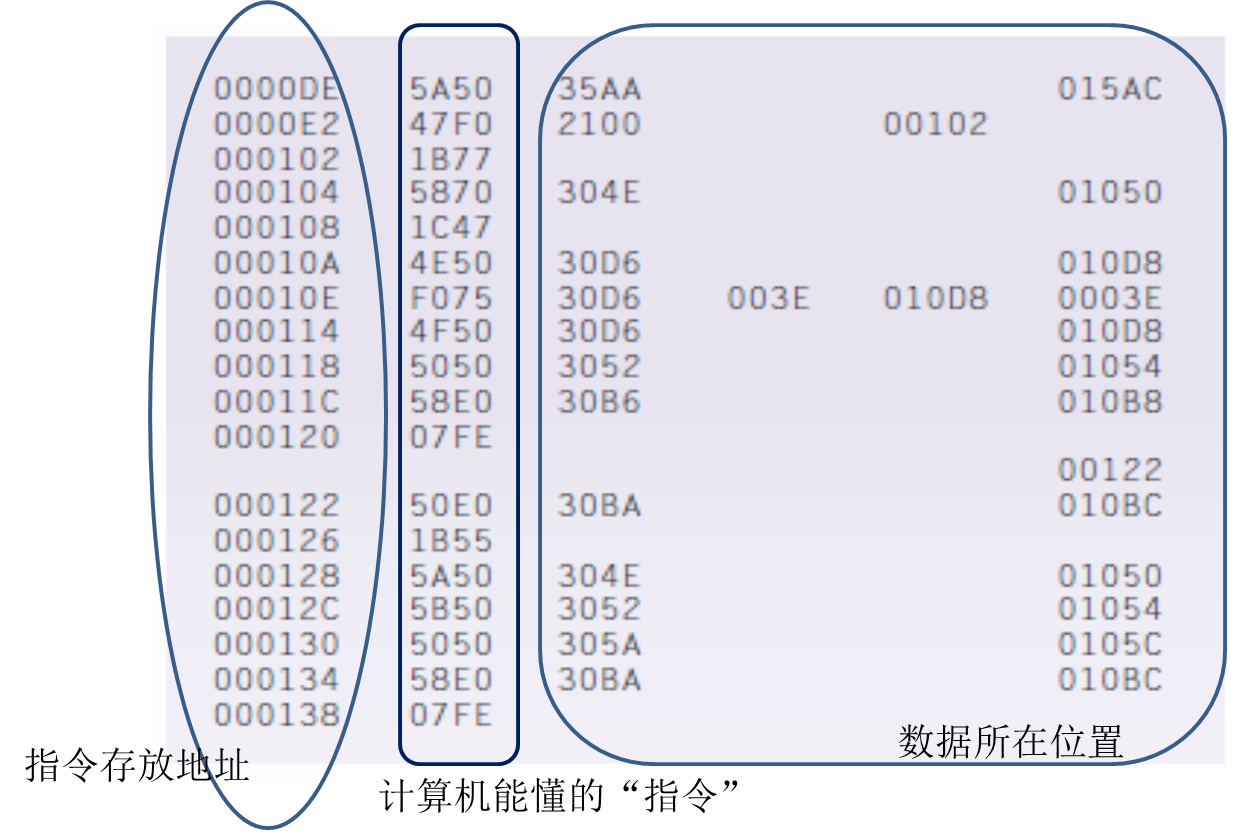
\includegraphics[scale=0.5]{4-programs/figs/prog-early.png}
	\caption{早期程序员的程序}
	\label{figs:prog-early}
	
\end{figure}

与程序对应的, 就是把``程序''放入计算机的存储里面的Von Neumann的体系结构. 相比于以前每一次写一个新程序就要重新去接线来说, 这样的内容确实简化了不少. Von Neumann构想的``计算机''应该由这四个内容组成: 内存(memory); 中央处理器(central processing unit): 其中包括控制单元(contol unit)和算术逻辑单元(arithematic logical unit, ALU), 分别控制按照规定的顺序执行以及计算其中可能的表达式; 以及输入输出设备(input/output devices). 

\begin{figure}[h!]
	\centering
	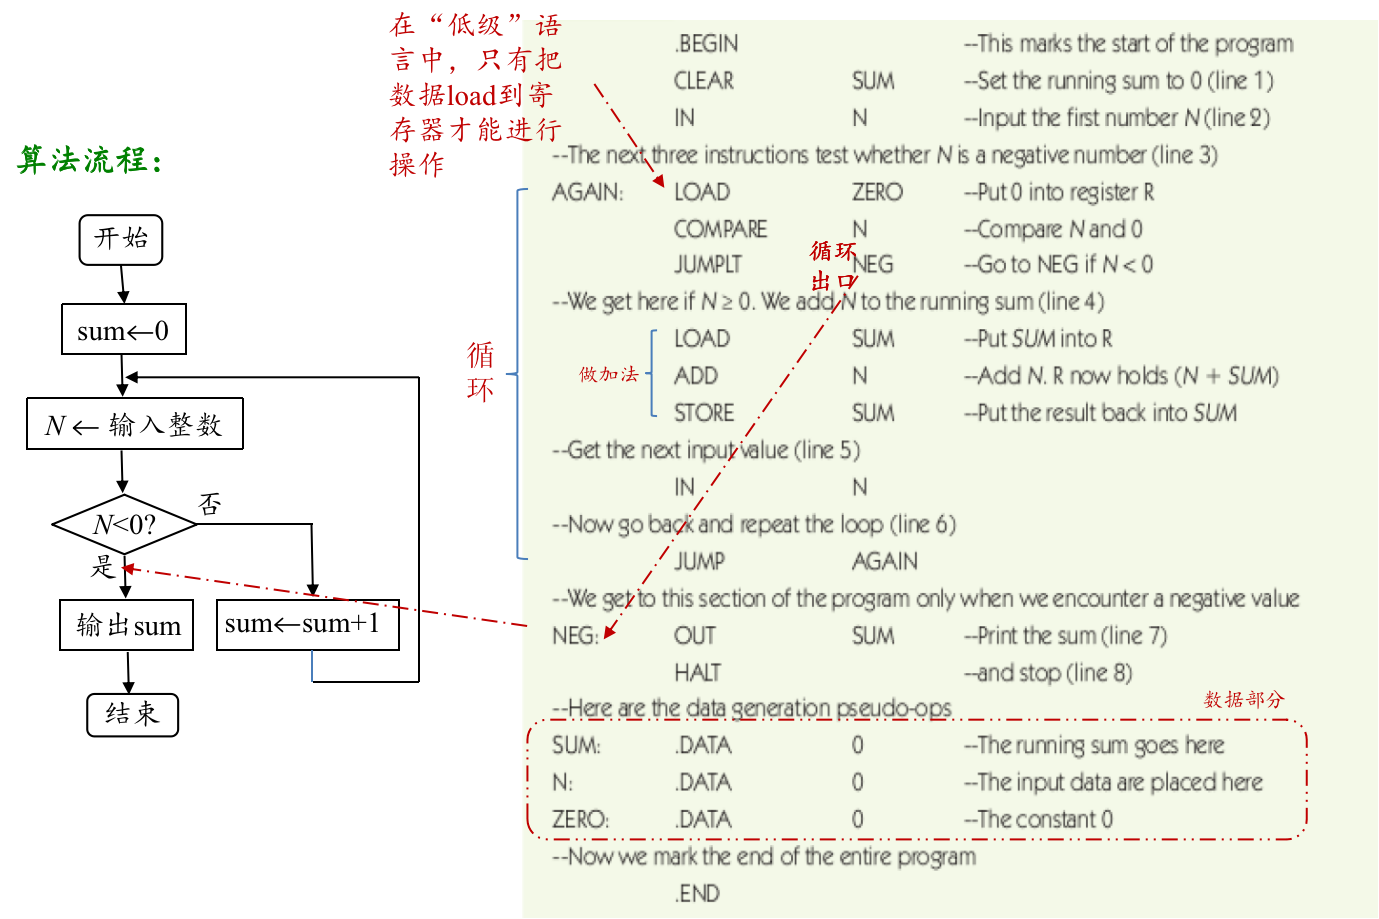
\includegraphics[scale=0.5]{4-programs/figs/asm-example.png}
	\caption{一段汇编指令 你能一眼看出来它想表达东西吗?}
	\label{figs:asm-eg}
	
\end{figure}

我们的计算机科学家很快就发现了这件事情很难办, 因为首先, 这一堆东西根本难以阅读. 聪明的计算机科学家采取了把那些抽象的数字和指令编号用一个一个比较直观的简单的记号, 这样一来就至少不会让我们感到头晕眼花了. 但是, 我们还是不知道这个程序到底要干什么. 比如我们要实现对输入的非负整数进行累加,遇到负数停止这样一个简单的操作, 我们可能需要写这样的程序, 见图\ref{figs:asm-eg}.

这就是我们为什么要使用高级的语言了. 由于项目变大的时候这些内容根本难以维护, 这就爆发了``软件危机''--越想改好, 但是bug越来越多. 

\begin{quote}
	The major cause of the software crisis is that the machines have become several orders of magnitude more powerful! To put it quite bluntly: as long as there were no machines, programming was no problem at all; when we had a few weak computers, programming became a mild problem, and now we have gigantic computers, programming has become an equally gigantic problem.
	
	\hfill --Edsger Dijkstra, The Humble Programmer (EWD340), Communications of the ACM
\end{quote}

人们感到十分的苦恼. 有没有一个更抽象的东西让我们把这些都机械化地管好呢? 其实是有的, 打败powerful computer的最好的办法就是设计一套规则, 让我们自动的管好这些我们不想理睬的power. 


我们期望的编程语言应该什么样? 相较于汇编语言直接与机器像婆婆妈妈那样事无巨细的吩咐好, 我们不妨想创建一个小管家, 让它可以帮助我们做得更加抽象一点, 比如: 

\begin{itemize}
	\item 程序员不需要关心数据究竟放在那里,也不必理会数据在存储器中的移动的细节;
	\begin{itemize}
		\item 这就是逻辑层面上关心的是“名”和“作用域”;
	\end{itemize}
	\item 程序员可以用“宏观”的视角,在“问题求解”的层次上看待计算任务,用于搭建“算法”的“block”可以相对大;
	\item 程序可以“跨平台”运行,即不“紧密”依赖于机器硬件;
	\item 尽量使用标准的数学表达形式,并让程序设计语言的语句更接近“自然语言”. 
\end{itemize}



下面我们来看一下从数据到算法, 我们经历了什么: 

\begin{prob}
	从输入的数值序列中清除 0. 
\end{prob}

一个非常直观的思想是: “逐个”检查每个元素,是0就删除。但如果从“思想”到“算法”的话, 还需要回答: 
\begin{itemize}
	\item 怎么“逐个”,比如从左向右
	\item 怎么“删除”,比如拿另外一个元素填入删除元素的位置
	\item 拿哪个元素来填,比如最“后面”一个
	\item 怎么控制“位置”
\end{itemize}

回答了这个问题, 我们可以提出``Converging-Pointer算法'':
采用两个“指针”,从序列两端相向移动,左指针管“检查”,右指针管“填空”,当两指针相遇时就到算法该结束的时候了。


好, 有了这个思想, 我们就可以写出如下的伪代码: 

\begin{lstlisting}
输入正整数n  // n是待清洗数据序列长度
数组data:=输入序列
legit:=n	// 有效数字计数器legit赋初值n
left:=0	// 当前检查位置指针left赋初值0
right:=n-1	// 当前序列末位置指针right赋初值n-1
while not(left>right) do //最后一次循环left=right
    if data[left]=0 then
        legit:=legit-1
        data[left]:=data[right]
        right:=right-1
    else
        left:=left+1
\end{lstlisting}


然后就可以写出C++的代码了. 

\begin{lstlisting}[language=c++]
while (left<right){
      if (data[left]!=0)
          left=left+1;
      else{
          legit=legit-1;
          data[left]=data[right];
          right=right-1;
       }
}
if (data[left]==0)  legit=legit-1;
	\end{lstlisting}


\ti{如何定义语言}

我们来看一下这份讲义, 我们日常生活中主要的语言: 汉语. 我们在高中的时候可能会了解: 这些句子的组成结构组成的汉语句子是符合语法的.  

\begin{lstlisting}
<句子>
<主语><动宾结构>
<主语><<谓语><宾语>>
<主语><谓语>
<主语><状语><谓语>
<主语><谓语><补语>
<名词><副词><动词><名词>
<名词><动词><补语>
王同学<动宾结构>
王同学学习<名词>
王同学<状语>学习数学
王同学<副词>学习数学
王同学努力地学习数学。
\end{lstlisting}

如果有的句子与没有出现在语法中, 如“王同学努力地数学学习”, 我们就可以认为这是语病, 写在作文里是要扣分的. 但是还有一类句子, 如“数学努力地学习王同学”, 虽然合乎语法, 但是并没有道理. 我们说这个矩阵不是“合理”的. 我们为什么会这么说? 因为我们关注了一个语言的两个重要的部分: 语法和语义(就像在第一章提到的一样). 既然两个都叫做``语言'', 那么他们的相似之处也不少, 程序设计语言和自然语言最大的不同在哪里?


其实, 程序设计语言是人专门``设计''出来的. 比如C++之父Bjarne Stroustrup, Java之父James Gosling. 目前, 维基百科上已经提到了有超过700种程序语言. 


要设计程序设计语言, 要拿出的心思更多应该在权衡上. 为什么这样说? 我们应该权衡什么? 首先要观察机器``能''或``不能''; 齐次要观察人类是不是方便. 作为一个机器, 其只是没有感情的工具, 因此我们必须要求语言完全没有歧义, 并且解释的规则是完全确定的. 什么是``规则''? 比如语言定义的两个要素:语法(什么样的形式是“合法”的?)和语义(合法的形式是什么意思?(例如:执行后会产生什么效果?))的精确定义\footnote{两者“规则”的精确描述难度差别非常大。}. 正是这样严苛的规则, 保证了``机器永远是对的''.

两个人用自然语言沟通,两个人都可能在语言使用上“出错”,但人和机器沟通,“出错”的一定是人。


 






